%%
%% This is file `mcmthesis-demo.tex',
%% generated with the docstrip utility.
%%
%% The original source files were:
%%
%% mcmthesis.dtx  (with options: `demo')
%%
%% -----------------------------------
%%
%% This is a generated file.
%%
%% Copyright (C)
%%       2010 -- 2015 by Zhaoli Wang
%%       2014 -- 2019 by Liam Huang
%%       2019 -- present by latexstudio.net
%%
%% This work may be distributed and/or modified under the
%% conditions of the LaTeX Project Public License, either version 1.3
%% of this license or (at your option) any later version.
%% The latest version of this license is in
%%   http://www.latex-project.org/lppl.txt
%% and version 1.3 or later is part of all distributions of LaTeX
%% version 2005/12/01 or later.
%%
%% This work has the LPPL maintenance status `maintained'.
%%
%% The Current Maintainer of this work is Liam Huang.
%%
%%
%% This is file `mcmthesis-demo.tex',
%% generated with the docstrip utility.
%%
%% The original source files were:
%%
%% mcmthesis.dtx  (with options: `demo')
%%
%% -----------------------------------
%%
%% This is a generated file.
%%
%% Copyright (C)
%%       2010 -- 2015 by Zhaoli Wang
%%       2014 -- 2019 by Liam Huang
%%       2019 -- present by latexstudio.net
%%
%% This work may be distributed and/or modified under the
%% conditions of the LaTeX Project Public License, either version 1.3
%% of this license or (at your option) any later version.
%% The latest version of this license is in
%%   http://www.latex-project.org/lppl.txt
%% and version 1.3 or later is part of all distributions of LaTeX
%% version 2005/12/01 or later.
%%
%% This work has the LPPL maintenance status `maintained'.
%%
%% The Current Maintainer of this work is Liam Huang.
%%
\documentclass[12pt]{mcmthesis}
\usepackage{float}
\usepackage{indentfirst} 
\usepackage{graphicx} 
\usepackage{subfigure}
\usepackage{multicol} 
\usepackage{cite}
\setlength{\parindent}{2em} 
\mcmsetup{CTeX = false,   % 使用 CTeX 套装时,设置为 true
        tcn = 2011260, problem = C,
        sheet = true, titleinsheet = true, keywordsinsheet = true,
        titlepage = false, abstract = true}
\usepackage{newtxtext}%\usepackage{palatino}
\usepackage{lipsum}
\title{A Wealth of Data}
\author{\small \href{http://www.latexstudio.net/}
  {
\includegraphics[width=7cm]{mcmthesis-logo}}}
\date{\today}
\begin{document}
\begin{abstract}
	\par Now is the era of e-commerce, in order to help companies gain an edge on e-commerce platforms, our team makes anlysis and identify key patterns, relationships, measures in past customer-supplied ratings and reviews.\\
	\indent \textbf{First}, we performed \textbf{data cleaning}. Because we do not consider emoticons  and find some HTML tags in the review body, we filter out emoticons and HTML tags. After processing the data, we discovered the quarterly nature of the three categories of goods and the relationship between star ratings and purchase intentions.\\
	\indent \textbf{Next} to identify data measures, we use \textbf{TF-IDF} and \textbf{sentiment analysis model} to build a review quality measurement function and modify it using the data of  vine  and verified\_purchase helpful\_votes and total\_votes.\\
	\indent \textbf{Then} in our time-based part, we use the comment quality measurement function with \textbf{Markov Chain} and chart discuss time-based measures and patterns to find the regular pattern of the rise and fall of reputation.  Reputation generally rises first, then falls and finally stabilized.\\
	\indent \textbf{Finally}, we analyzed the statistics and found that specific star ratings did not significantly cause more reviews and some specific quality descriptors of textbased reviews are strongly associated with rating levels.
\begin{keywords}
Data Cleaning; TF-IDF; Sentiment Analysis Model; Markov Chain
\end{keywords}
\end{abstract}
\maketitle
%% Generate the Table of Contents, if it's needed.
\tableofcontents
\newpage
%%
%% Generate the Memorandum, if it's needed.
% \memoto{\LaTeX{}studio}
% \memofrom{Liam Huang}
% \memosubject{Happy \TeX{}ing!}
% \memodate{\today}
% \logo{\LARGE I'm pretending to be a LOGO!}
% \begin{memo}[Memorandum]
%   \lipsum[1-3]
% \end{memo}
%%

\section{Overview}
\subsection{Background}
\indent This era is the era of data. Everyone's life is inseparable from data, just as McKinsey , a global well-known consulting company, said: “Today, Data has penetrated into every industry and business function area, and has become an important production factor. The mining and application of massive data indicates a new wave of productivity growth and the coming of consumer surplus.”\\
\indent One of the most widely used area of data today is the e-commerce platform. Merchants are always receiving feedback from their consumers about their product. The purpose of this essay is to establish an effective and reliable evaluation mechanism from the data obtained by merchants, thereby helping both to increase the sales volume of the merchants and to make consumers have a better shopping experience.\\
\subsection{Problem Summary}
\par 1. Clean the data set: remove misleading data and irrelevant data from the data set to ensure that the data we analyze and process afterwards are all valid data.

\par 2. Quantify the consumer's text-based reviews, and then integrate the star ratings and reviews of the consumer to establish a comprehensive product evaluation standard.

\par 3. Build a function to reflect the impact of early consumer's review of products on the product's future reputation.

\par 4. Determine the impact of early customer's star rating on later customer's review of the product.

\par 5. Determine whether specific quality descriptors are associated with rating levels or not.
%\subsection{Syntax (how to type \LaTeX\ commands --- these
%  are the rules)}
%
%\lipsum[3]
%\begin{itemize}
%\item the angular velocity of the bat,
%\item the velocity of the ball, and
%\item the position of impact along the bat.
%\end{itemize}
%\lipsum[4]
%\emph{center of percussion} [Brody 1986], \lipsum[5]
%
%\begin{Theorem} \label{thm:latex}
%\LaTeX
%\end{Theorem}
%\begin{Lemma} \label{thm:tex}
%\TeX .
%\end{Lemma}
%\begin{proof}
%The proof of theorem.
%\end{proof}
%
%\subsection{Other Assumptions}

%\begin{figure}[h]
%\small
%\centering
%
\includegraphics[width=8cm]{example-image-a}
%\caption{The name of figure} \label{fig:aa}
%\end{figure}

\section{Assumption and Justification}
To simplify our model, we make the following assumptions, each of which is properly justified. 
\begin{enumerate}
	\item The consumers counted in the data set is a random sample of all consumers in reality so that the analysis results of the data set can directly reflect the responses of all consumers and provide reliable information for the company.
	
	%\item All the reviews and star ratings reflect the true attitude and experience of consumers. There are neither malicious reviews by malicious people nor those who were hired by the companie to provide positive reviews.
	
	\item The sales of the product is proportional to the number of reviews.
\end{enumerate}

%\lipsum[8] \eqref{aa}
%\begin{equation}
%a^2 \label{aa}
%\end{equation}
%
%\[
%  \begin{pmatrix}
%  {a_{11} } & {a_{12} } & {a_{13} }  \\
%  {a_{21} } & {a_{22} } & {a_{23} }  \\
%  {a_{31} } & {a_{32} } & {a_{33} }  \\
%  \end{pmatrix}
%  = \frac{{Opposite}}{{Hypotenuse}}\cos ^{ - 1} \theta \arcsin \theta
%\]
%\lipsum[9]
%
%\[
%  p_{j}=\begin{cases} 0,&\text{if $j$ is odd}\\
%  r!\,(-1)^{j/2},&\text{if $j$ is even}
%  \end{cases}
%\]
%
%\lipsum[10]
%
%\[
%  \arcsin \theta  =
%  \mathop{{\int\!\!\!\!\!\int\!\!\!\!\!\int}\mkern-31.2mu
%  \bigodot}\limits_\varphi
%  {\mathop {\lim }\limits_{x \to \infty } \frac{{n!}}{{r!\left( {n - r}
%  \right)!}}} \eqno (1)
%\]

\section{Notation}
We use the following symbols in our model and analysis for convenience, cf. Table 1.
\begin{table}[H]
	\centering
	\setlength{\tabcolsep}{8mm}
	\caption{Symbols and its description}
	\begin{tabular}{cl}
				\hline
				{\bf Symbol} &   \multicolumn{1}{c}{\bf Meaning} \\
				\hline
				{\bf $i$ } & Corresponding item number\\ 
				
				{\bf $r$} & The review that we process\\
				
%				\multirow{2}{*}
				{\bf $F_{i}$ } & The frequency of a word appears in all reviews of item i\\
				
				{\bf $T_{i}$ } & The total number of words in all reviews of item i \\
				
				{\bf $\alpha$} &  The frequency of a word that was used in daily life \\
				
				{\bf $S$} &  A number that quantify whether a word is neutral or not\\
				
				{\bf $R(r)$ } & Function that quantify the quality of the content of review r \\
				
				{\bf $A_{i}$ } & How many time that a word appears in all reviews of item i \\
				
				{\bf $Q(r)$} & The function that quantify review r \\
				
				{\bf $M_{i}(p)$} &  The function that measure product p in item i based on both review and star rating \\
				
				{\bf $S_{r}$ } & The star rate of review r \\
				
				\hline
	\end{tabular}
\end{table}

\section{Problem 1}
In this section, we focus on clean the data that was provided, and identifying useful information from the data in order to help the company succeed in the future product launch.

\subsection{Data cleaning}
Go through the data provided and find that there are some emojis which are not a part of ASCII characters in the reviews and some HTML tags that maybe crawled from the Amazon website using crawling technology.

In both cases, it is inconvenient for us to analyze and process the data, and such data are not critical information in reviews, so we need to clean up the data. We identified those entries that need to be modified from the data, and then rearrage it to complete the cleaning of data.

\subsection{Useful information}
We identified two kinds of useful information based on the star ratings, reviews, and helpfulness ratings. The first useful information is the change of product sales with months. We divided the time of the review into months, and use the total number of reviews in this months as the sales of the product, and obtained the following information.
\begin{figure}[htbp]
	\centering
	\subfigure[Microwave oven]{
		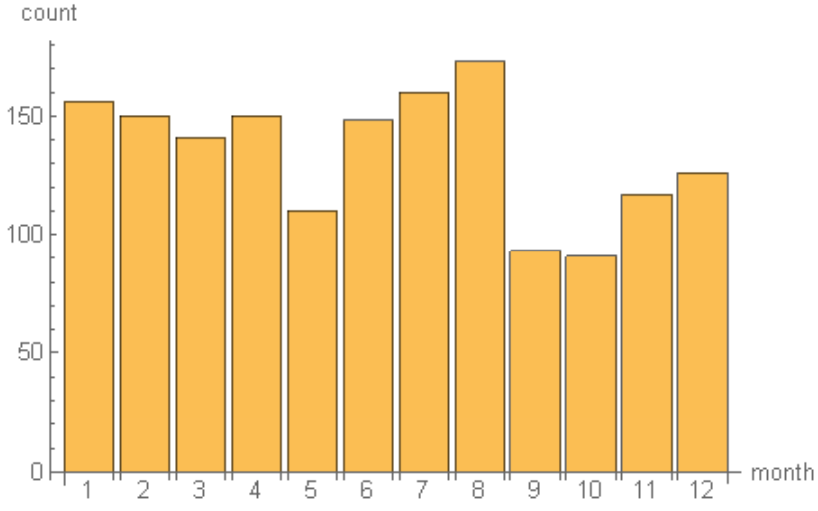
\includegraphics[width=7cm,height=7cm]{figures/m-season.png}
	}
	
	\quad
	\subfigure[Pacifier]{
		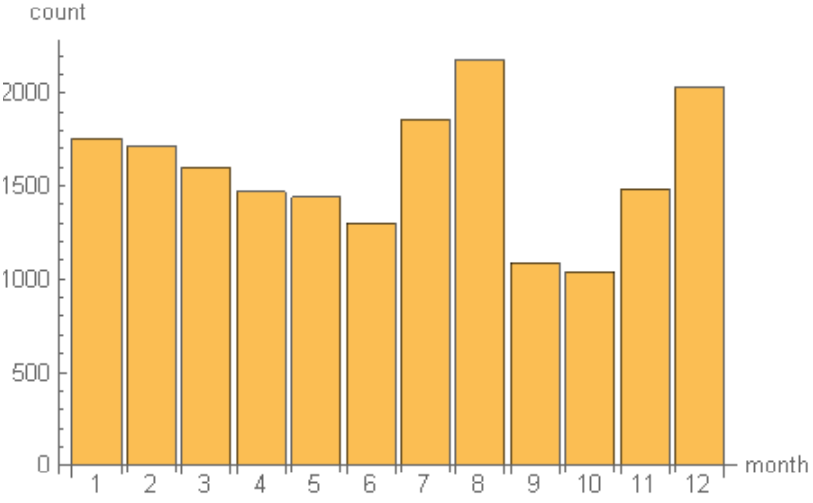
\includegraphics[width=7cm,height=7cm]{figures/p-season.png}
	}
	
	\quad
	\subfigure[Hair dryer]{
		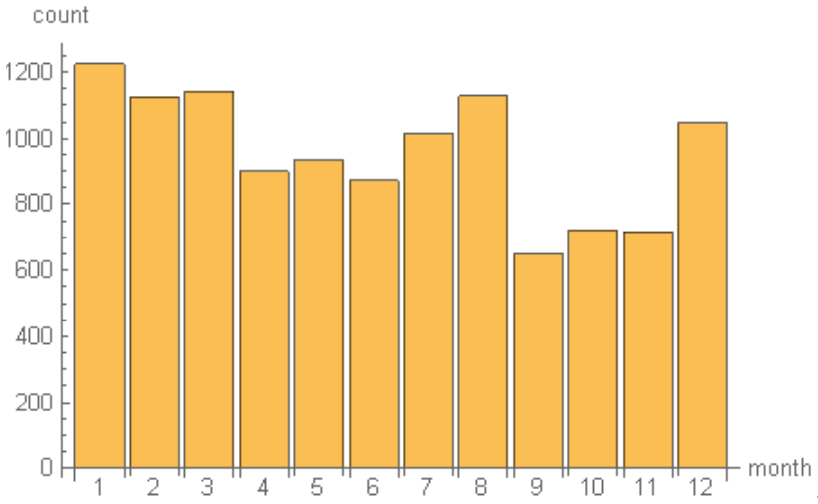
\includegraphics[width=7cm,height=7cm]{figures/h-season.png}
	}
	
	\caption{Sales in different month}
\end{figure}
\newpage
We can see that the three types of goods will have higher sales in January, February, July, August, and December, also lower sales in May, June, September, and October.

The second useful information we identified is to show merchants what kind of reviews buyers will be used to influence their willingness to buy the product. We use helpfulness ratings, star ratings and the number of reviews to establish a three-dimensional coordinate chart.

\begin{figure}[htbp]
	\centering
	\subfigure[Microwave oven]{
		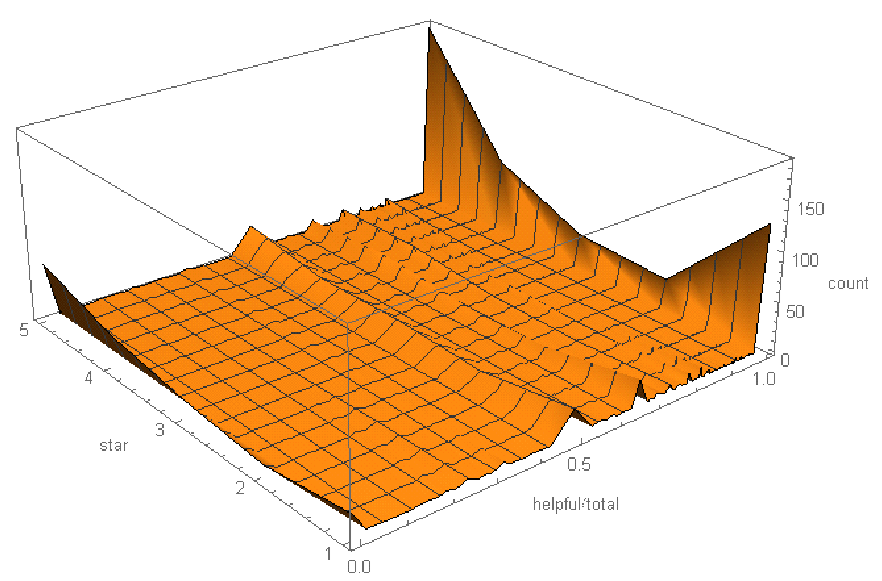
\includegraphics[width=9cm,height=6cm]{figures/m-3.png}
	}
	
	\quad
	\subfigure[Pacifier]{
		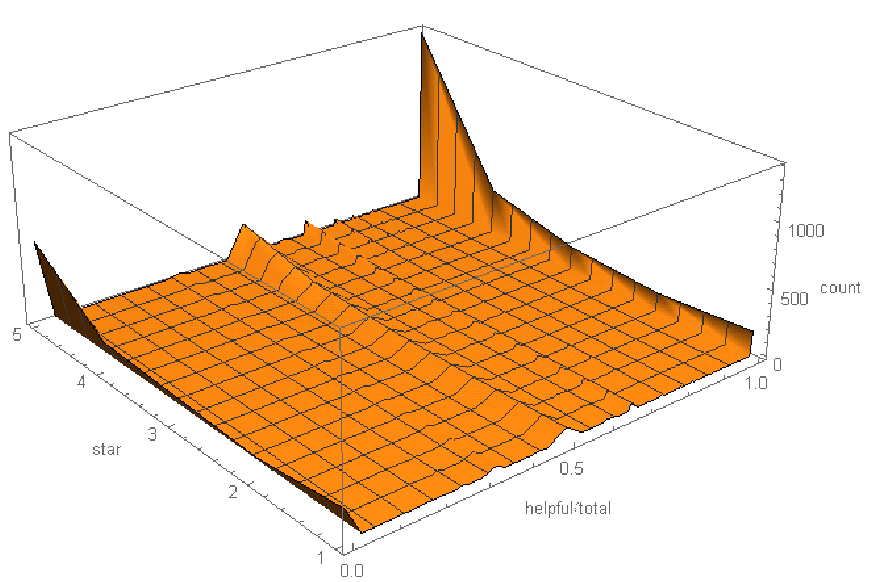
\includegraphics[width=9cm,height=6cm]{figures/p-3.png}
	}
	
	\quad
	\subfigure[Hair dryer]{
		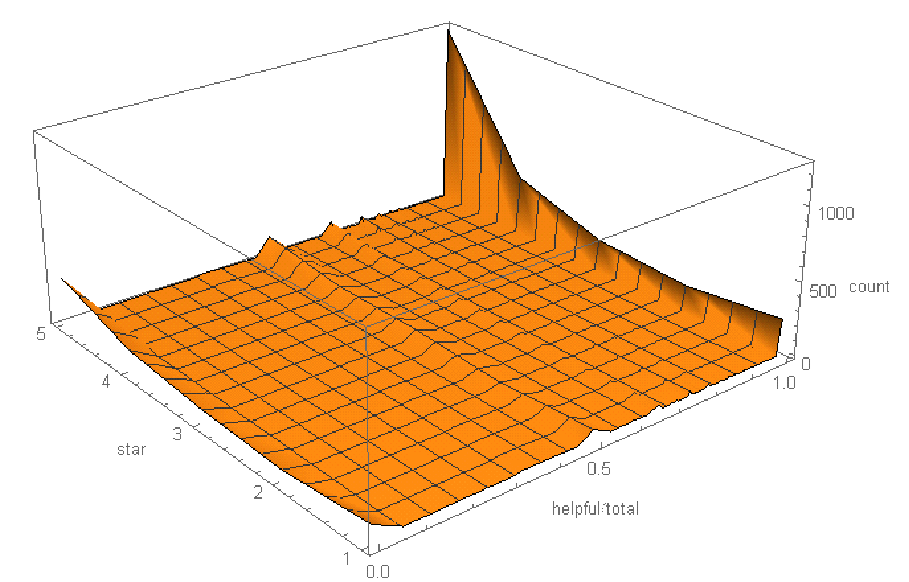
\includegraphics[width=9cm,height=6cm]{figures/h-3.png}
	}
	
	\caption{Useful Information}
\end{figure}
\newpage
We can see that the four corners in the image are much more higher. It shows that people are more willing to decide whether to buy this product based on the content of one-star and five-star reviews. The content of reviews did not influence people's buying decisions that much.


\section{Problem 2}

\subsection{Question a}
In this section, we want to establish a comprehensive evaluation indicator based on star ratings and product reviews. Prior to this, because consumer reviews of products were written data, it was not conducive to our quantitative analysis of products, so we needed to rate customer reviews of products similar to star ratings.

First, we use an algorithm called TF-IDF to quantify the content of the review $r$. \cite{1} To accomplish such a goal we need to calculate the frequency of each word appears in comment $r$ by the following formula$$F_{i}=\frac{A_{i}}{T_{i}}$$


Because although some words appear relatively frequently, they have no practical meaning, so we multiply the calculated word frequency by a parameter related to the frequency of the word in daily life to reflect the word's importance in the review $r$. After calculating the importance of the vocabulary, the word is multiplied by its sentimental analysis coefficient $S$ \cite{2} to reflect the attitude of the consumer. Finally, all the words in review $r$ are similarly processed and then summarized to quantify the content of the review. The function is as follow$$R(r)=\sum F_{i} * \log \frac{1}{\alpha} * S$$

After quantifying the content of the review, we need to quantify the review as a whole, including consider whether the review is helpful, whether the reviewer is an Amazon Vine member and whether the reviewer has been verified for the purchase. To make our description clearer, we temporarily define a function $E(r)$ as follow $$E(r)=\frac{\text { helpful\_votes }}{\text { total\_votes }} * R(r)$$

For those reviews whose total\_vote is zero. We use the average $\frac{\text { helpful\_votes }}{\text { total\_votes }}$ of all those reviews whose total\_vote is not zero to replace the $\frac{\text { helpful\_votes }}{\text { total\_votes }}$ in the function above.

Now we define the function $Q(r)$ that quantify review r like this $$Q(r)=E(r) *\left\{\begin{array}{ll}
\text { Vinetrue } \\
\text { VineFalse }
\end{array}\right.*
\left\{\begin{array}{ll}
\text { Verified } \\
\text { NotVerified }
\end{array}\right.$$

Vineture is defined as the average of $E(r)$ of all the reviews that was wrote by Amazon Vine member and other situation are defined similar like this.

Finally, we are able to define our data measure that based on ratings and reviews as follow$$M_{i}(i)=\frac{\sum Q(r) * S_{r}}{\sum Q(r)}$$

We draw the image with the number of reviews as the abscissa and the product level calculated by the function we established as the ordinate. Each point in the image represents a product
\begin{figure}[htbp]
	\centering
	\subfigure[Microwave oven]{
		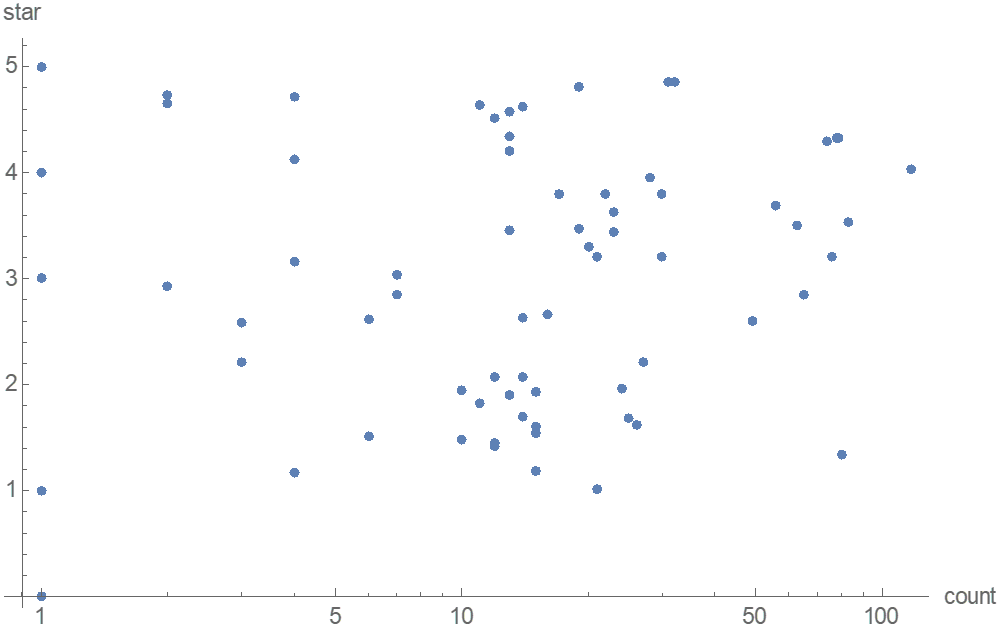
\includegraphics[width=7cm,height=7cm]{figures/m.png}
	}
	\subfigure[Microwave oven difference]{
		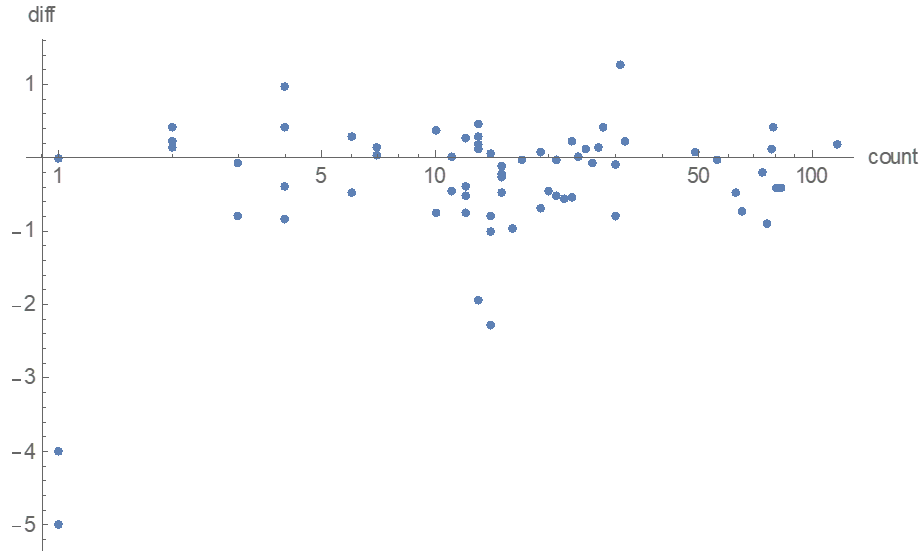
\includegraphics[width=7cm,height=7cm]{figures/m-1.png}
	}
	\quad
	\subfigure[Pacifier]{
		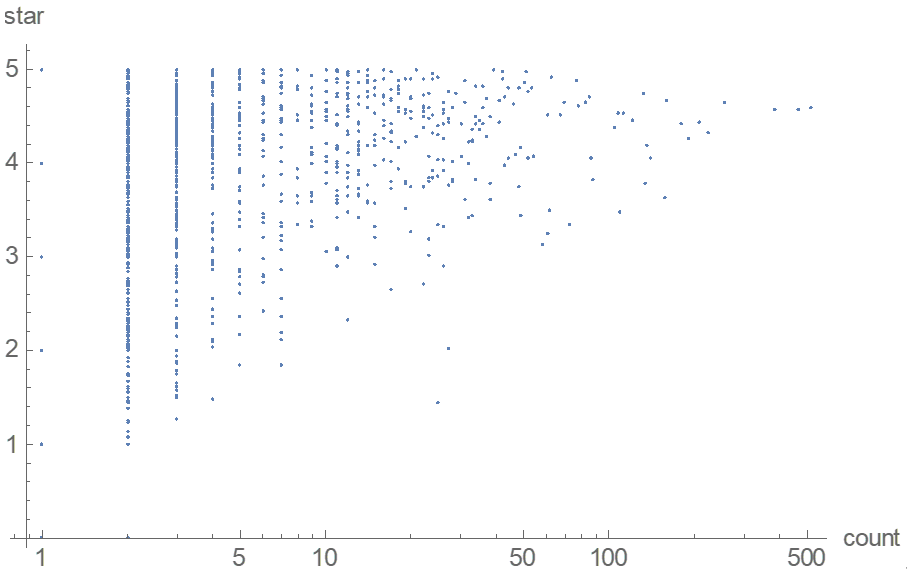
\includegraphics[width=7cm,height=7cm]{figures/p.png}
	}
    \subfigure[Pacifier difference]{
    	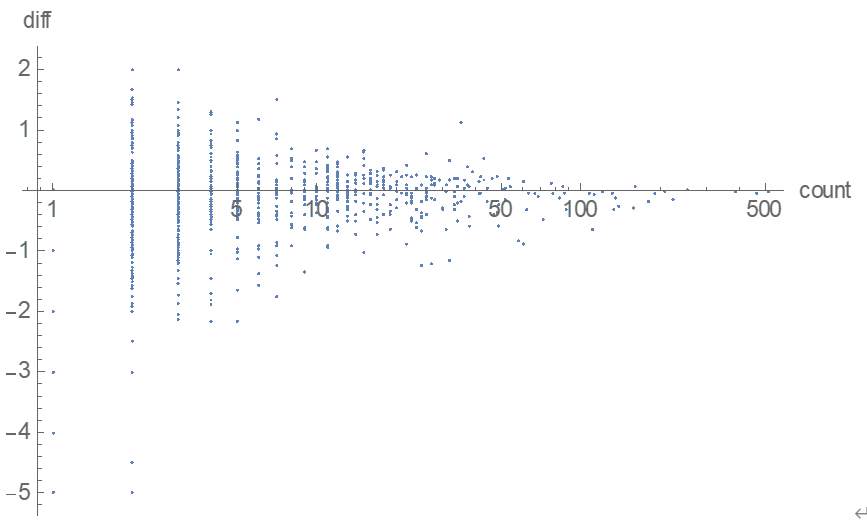
\includegraphics[width=7cm,height=7cm]{figures/p-1.png}
    }
	\quad
	\subfigure[Hair dryer]{
		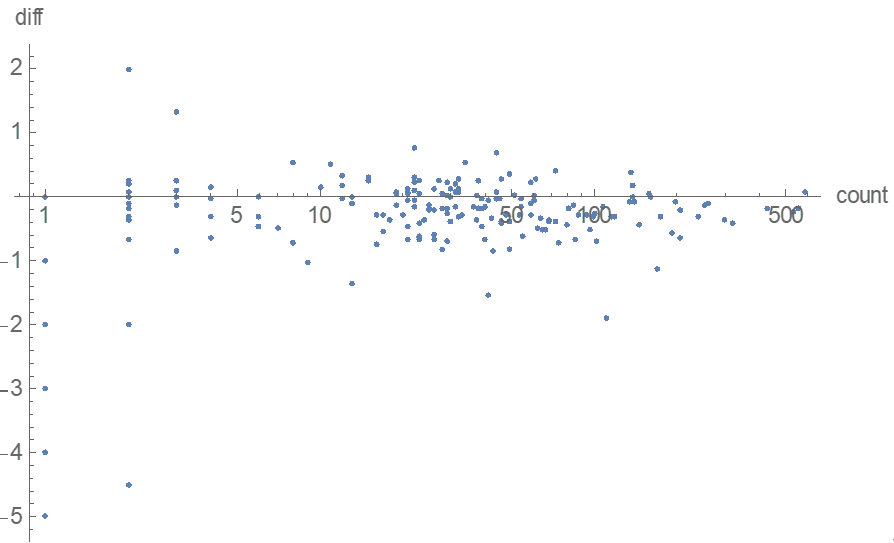
\includegraphics[width=7cm,height=7cm]{figures/h-1.png}
	}
    \subfigure[Hair dryer difference]{
    	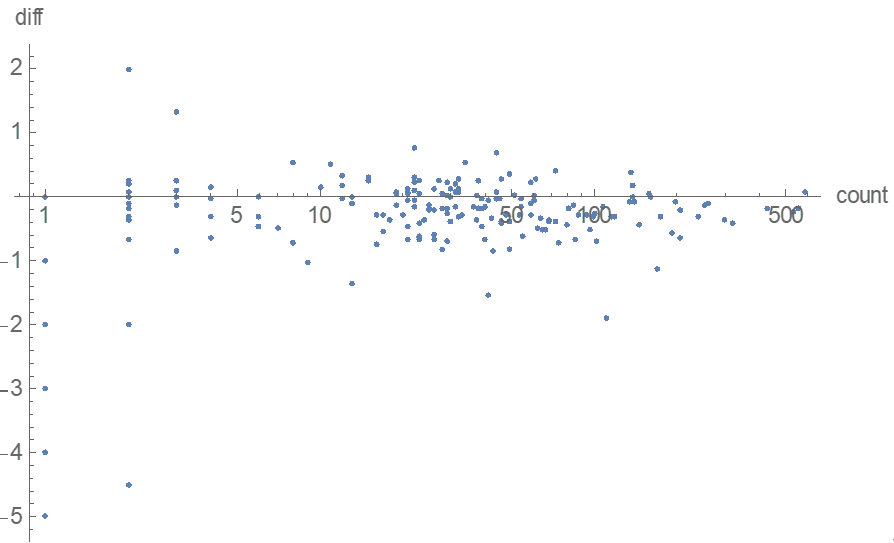
\includegraphics[width=7cm,height=7cm]{figures/h-1.png}
    }
	\caption{The result of our function}
\end{figure}
\newpage
From the figure we can see that if the number of the reviews is small, our measure function have a better measure since we take into the consideration in the quality of review. When the number of the review is large, our measure function have similar result with the average star rating one. But since we reduce the weight of lower quality review, it will have a more accurate result.
\subsection{Question b}
Our purpose in this section is to identify and discuss patterns that can represent the reputation of a product over time. Here we have identified two patterns, which are discussed separately below.
\begin{itemize}
	\item The first patterns we identified is based on Markov Chain Approch\cite{3}. First, we make a premise to ensure that the Markov Chain Approch can be used on the provided data set. This assumption is that the future reputation of the product will depend on the current reputation and do not care about how the current reputation is achieved. Based on this assumption, we separately process the microwave oven, pacifier, and hair dryer as follows:
	\begin{enumerate}
		\item Use one day as a basic time unit. Calculate how long has it been from the time the product's first review appear to this current moment.
		
		\item Use the functions $Q(r)$ and $M_{i}(p)$ we established in question a to calculate the score of the product based on all the reviews up to this moment, and use this as the reputation of the product at the current moment.
		
		\item Combine the above two values into a value pair, use the Markov Chain Approch to process these value pairs, and obtain the state change transformation matrix.
		
		\item The matrix of the initial status of the product reputation (the proportion of 1 to 5 evaluations) and the state transition matrix indicate the trend of the product's future reputation.(The first matrix below is the Initial Probabilities Matrix, the second martix is the Transition Matrix)
	\end{enumerate}
    The result of microwave oven:
    
    $$\left(\begin{array}{c}
    0.2625 \\
    0.0125 \\
    0.175 \\
    0.25 \\
    0.3
    \end{array}\right) , \left(\begin{array}{ccccc}
    0.875776 & 0.0993789 & 0. & 0.0124224 & 0.0124224 \\
    0.0546448 & 0.896175 & 0.0382514 & 0.00546448 & 0.00546448 \\
    0.0033557 & 0.0369128 & 0.922819 & 0.033557 & 0.0033557 \\
    0.00184162 & 0.00552486 & 0.0313076 & 0.93186 & 0.0294659 \\
    0. & 0.0104895 & 0.0104895 & 0.0839161 & 0.895105
    \end{array}\right)$$

    The result of pacifier:
    
    $$\left.\left(\begin{array}{c}
    0.159981 \\
    0.0495218 \\
    0.072817 \\
    0.147794 \\
    0.569886
    \end{array}\right) , \left(\begin{array}{ccccc}
    	0.344371 & 0.172185 & 0.0860927 & 0.0993377 & 0.298013 \\
    	0.0283019 & 0.613208 & 0.273585 & 0.0849057 & 0 \\
    	0 . & 0.0255517 & 0.821138 & 0.14518 & 0.00813008 \\
    	0.0002331 & 0.0027972 & 0.0205128 & 0.92634 & 0.0501166 \\
    	0.00098668 & 0.00378227 & 0.0101957 & 0.0613386 & 0.923697
    \end{array}\right)\right.$$
    
    The result of hair\_dryer:
    
    $$\left.\left(\begin{array}{c}
    0.128253 \\
    0.0594796 \\
    0.0762682 \\
    0.20632 \\
    0.52974
    \end{array}\right) , \left(\begin{array}{ccccc}
    0.553191 & 0.234043 & 0.0851064 & 0.0425532 & 0.0851064 \\
    0.00647948 & 0.941685 & 0.0410367 & 0.00431965 & 0.00647948 \\
    0.000835422 & 0.00835422 & 0.927318 & 0.0618212 & 0.00167084 \\
    0.000156617 & 0.000626468 & 0.0129992 & 0.974471 & 0.0117463 \\
    0.000533049 & 0.0019661 & 0.00266525 & 0.0692964 & 0.926439
    \end{array}\right)\right.$$
	\item Because the premise assumptions of the Markov Chain Approch, the result above can only show us the future trends of product's reputation. Since we cannot see how the product's reputation changes over time, we identified another pattern. At the every time unit, we use the function established by question a to calculate the scores of the subordinate products of each category of good, and then take an average of the ratings of these subordinate products as the reputation of this category of good, and then draw a reputation-time curve to see how the product's reputation change over time.
\begin{figure}[htbp]
	\centering
	\subfigure[Microwave oven]{
		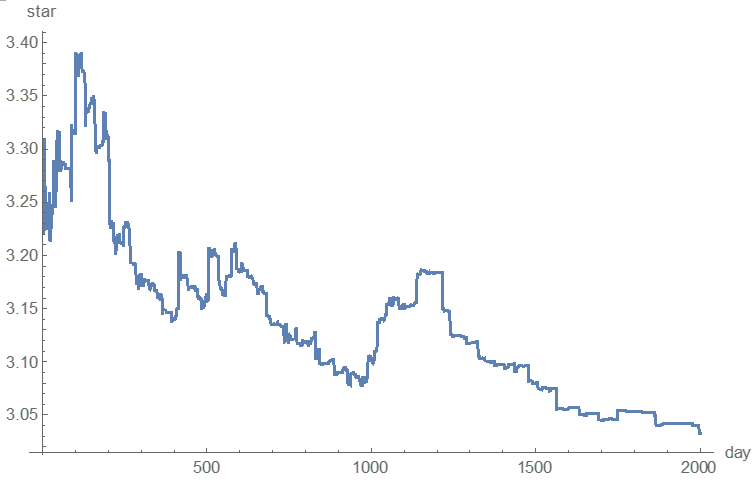
\includegraphics[width=7cm,height=7cm]{figures/m-time.png}
	}
	
	\quad
	\subfigure[Pacifier]{
		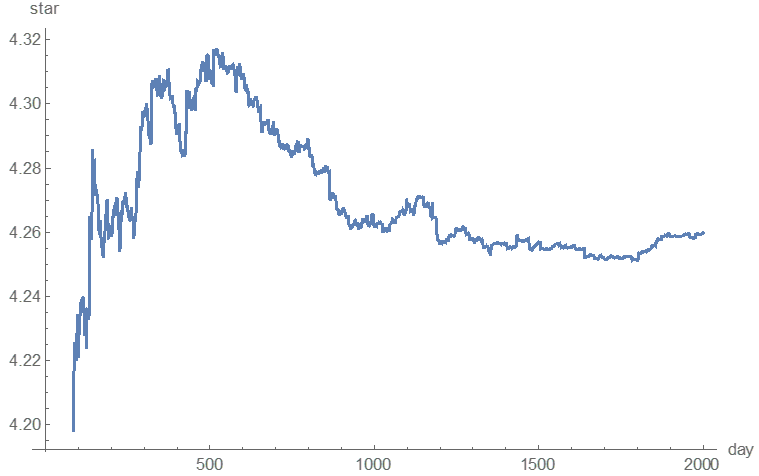
\includegraphics[width=7cm,height=7cm]{figures/p-time.png}
	}
	
	\quad
	\subfigure[Hair dryer]{
		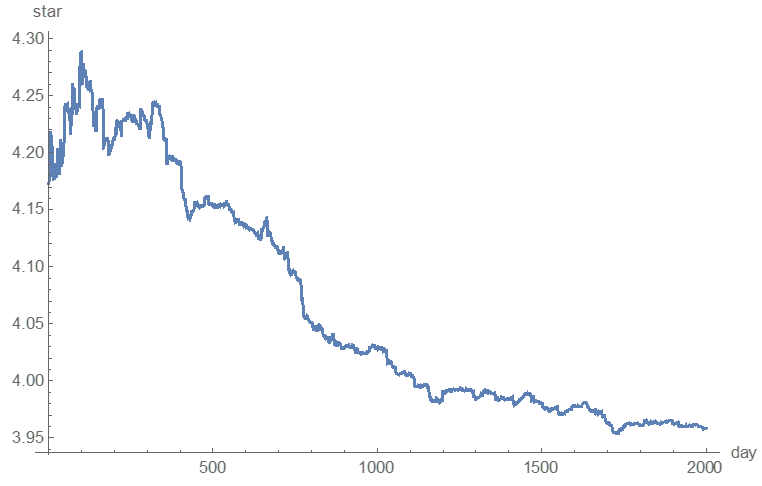
\includegraphics[width=7cm,height=7cm]{figures/h-time.png}
	}
	
	\caption{The trend of product's reputation}
\end{figure}
\newpage
	From the curve changes in the figure, we can see that the reputation changes of the three types of goods have common characteristics. Their reputations are all rose at first, then fell, and finally stabilized which matches the result of Markov Chain Approch that the star rating tend to stay the same with the maximum probability.
\end{itemize}

\subsection{Question c}
The purpose of this section is to find a combination of text-based reviews and star ratings to most accurately predict the future success or failure of a product. In order to achieve this goal, we need to use the function $M_{i}(p)$ we established in Question a as a measure of the reputation of product p, and finally use the value of $M_{i}(p)$ to measure the success of product p. According to the definition of the $M_{i}(p)$, it can be see that the value of $M_{i}(p)$ is related to the reviews of product p. So we consider the effect of a review r on the reputation of the product p. The average star rating of all reviews before review r is defined as $s_{prev}$, and $q_{prev}$ is defined as the average value of all reviews before review r using the function Q in question a. Assuming the star rating of review r is $s$ , then the new reputation of the product is as follows$$M_{new}=\frac{s_{prev}*q_{prev}+s*Q(r)}{q_{prev}+Q(r)}$$
So the difference of the new $M_{i}(p)$ and the old $M_{i}(p)$ caused by review r is $$\Delta M=\left|M_{\text {new }}-M_{\text {old }}\right|$$

When $\Delta M$ is larger than 0.1(we come up with this value by analysis all the data in the data set and choose a proper value), we can say that this review r has a great impact in predict whether this product is going to success or not. After exam all the reviews, we found that for each review r of microwave oven, pacifier, hair\_dryer,when $Q(r)$ is larger than 0.495908, 0.382742, 0.210319 respectively, if the star rate of review r is 4-5, then this review indicate that the product is more likely to success, if the star rate of review r is 1-2, then this review indicate that the product is more likely to fail.

\subsection{Question d}
In this section, we need to determine whether the star rating of the product by the early consumers will affect the product's review wrote by later consumers. We will discuss the different star ratings separately. For example, for one-star reviews, we count all reviews within a period of time after each one-star review (here we choose 7 days and 30 days). Categorize the reviews based on their star rating. We use the percentage of the corresponding star-rate reviews to all the reviews in this period as the ordinate to make the chart shown below.
\begin{figure}[htbp]
	\centering
	\subfigure[Microwave oven-7days]{
		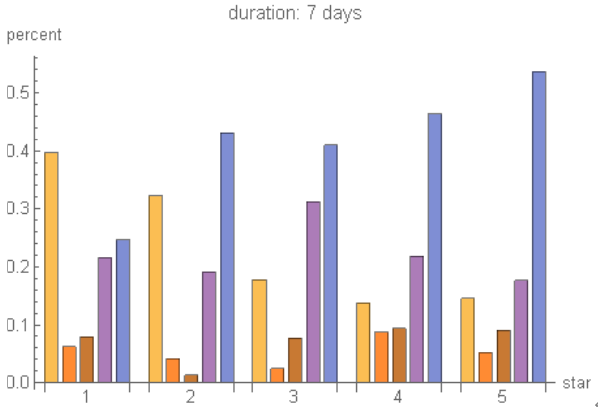
\includegraphics[width=5cm,height=5cm]{figures/m-7.png}
	}
	\subfigure[Microwave oven-30days]{
		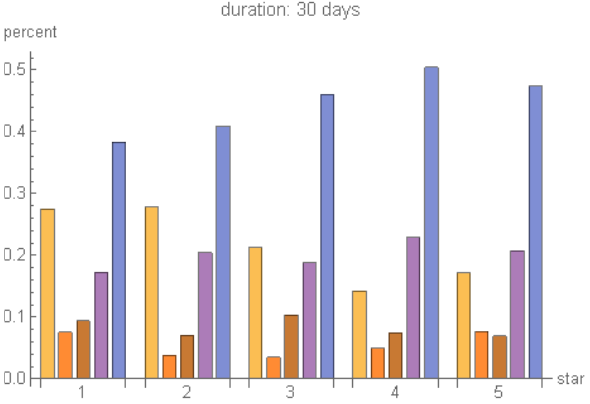
\includegraphics[width=5cm,height=5cm]{figures/m-30.png}
	}
	
	\quad
	\subfigure[Pacifier-7days]{
		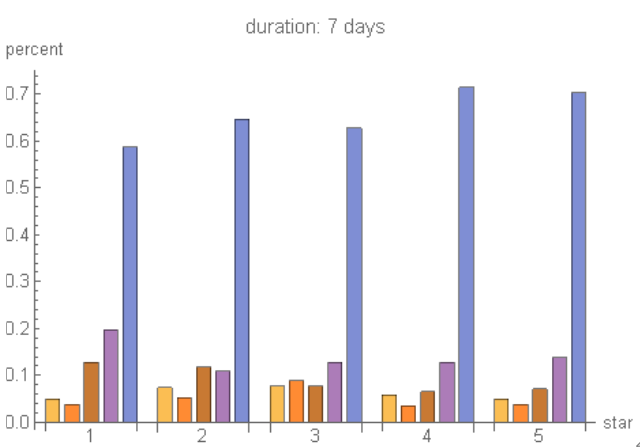
\includegraphics[width=5cm,height=5cm]{figures/p-7.png}
	}
	\subfigure[Pacifier-30days]{
		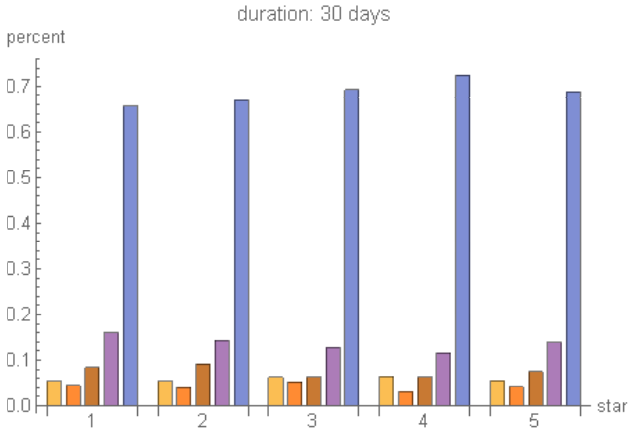
\includegraphics[width=5cm,height=5cm]{figures/p-30.png}
	}
	
	\quad
	\subfigure[Hair dryer-7days]{
		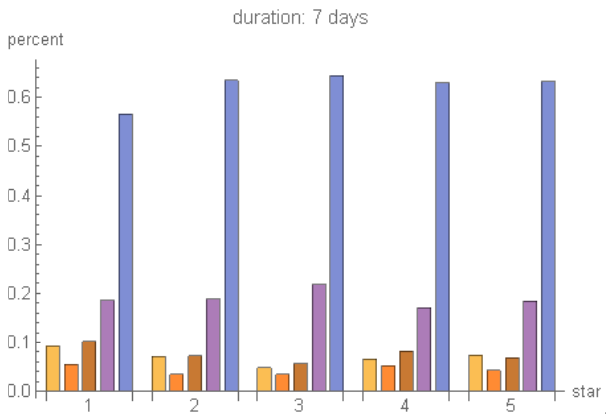
\includegraphics[width=5cm,height=5cm]{figures/h-7.png}
	}
	\subfigure[Hair dryer-30days]{
		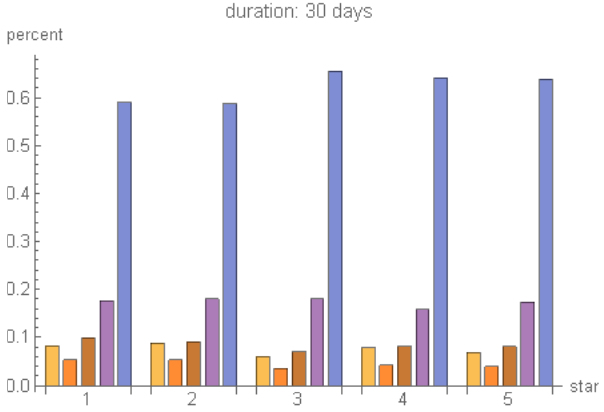
\includegraphics[width=5cm,height=5cm]{figures/h-30.png}
	}
\end{figure}
\newpage
From the charts we can see that when people see more higher star rating, they tend to give higher reviews, and when they see more lower star rating, they tend to give lower reviews.And low star rating review about microwave oven will cause stronger agreement than the cases in pacifier and hair dryer.
\subsection{Question e}
In this section, we explore the relationship between some special words in the reviews and the star ratings given to the products by the consumers. In order to achieve our goal, we first need to pre-process product reviews, including removing duplicate reviews, to ensure the authenticity and reliability of subsequent review processing. After that, we split the complete comment into individual words. It is inevitable that there will be certain stopwords in each comment. These words appear frequently in the comments, but they do not contain actual meaning and will affect our subsequent analysis. Therefore, we will match the words we obtained with the Natural Language Toolkit's stopword library to remove stopwords from the comments. So far, the words in the reviews can more or less indicate consumer opinions and descriptions of the product.

In order to select the most informative word from these words, we perform the following processing on each word: first we add the star ratings corresponding to all reviews containing this word, and then use this sum value to divide the number of comments that contain this word. Then use this value and the number of comments that contain this word as the measure of the word. After that, we use these two indicators as standard to sort the words from large to small, and select the words with the highest ranking in the two indicators from the results of the ranking. Now we can be sure that these words contain most information about star ratings.

At this point, we have successfully located so called "specific quality descriptors". We counted the number of reviews containing these words in each level of star and plotted the following chart

\begin{figure}[htbp]
	\centering
	\subfigure[Positive Words]{
		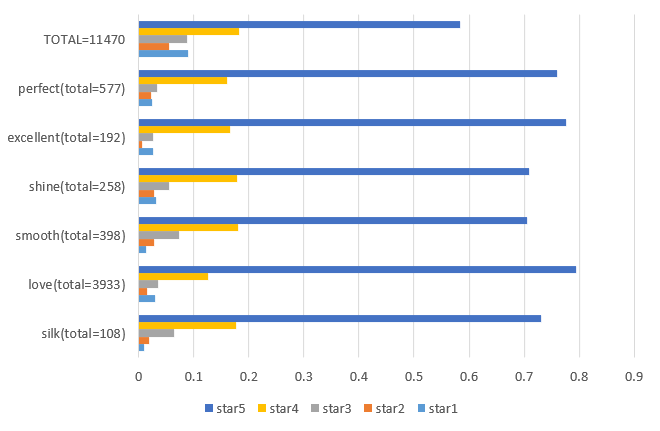
\includegraphics[width=5cm,height=5cm]{figures/pos-h.png}
	}
	\subfigure[Negative words]{
		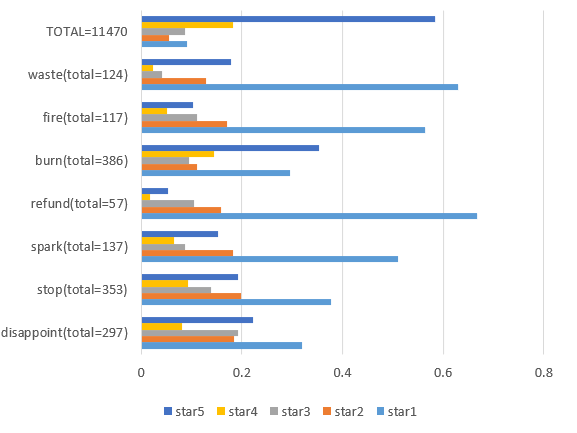
\includegraphics[width=5cm,height=5cm]{figures/neg-h.png}
	}
	\caption{Hair\_dryer}
\end{figure}

\begin{figure}[htbp]
	\centering
	\subfigure[Positive Words]{
		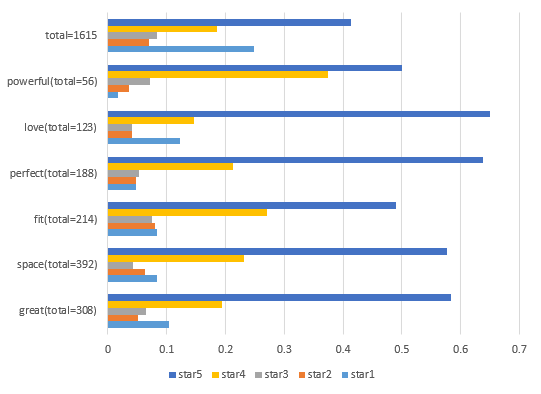
\includegraphics[width=5cm,height=5cm]{figures/pos-m.png}
	}
	\subfigure[Negative words]{
		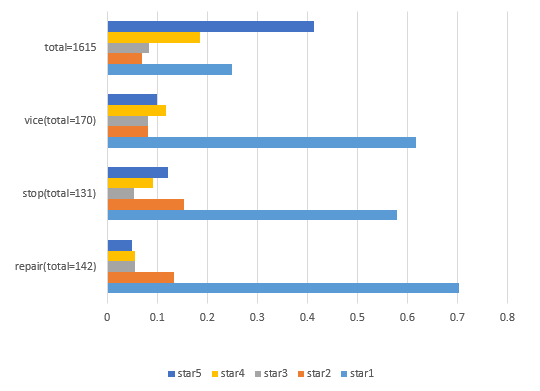
\includegraphics[width=5cm,height=5cm]{figures/neg-m.png}
	}
	\caption{Microwave oven}
\end{figure}

\begin{figure}[htbp]
	\centering
	\subfigure[Positive Words]{
		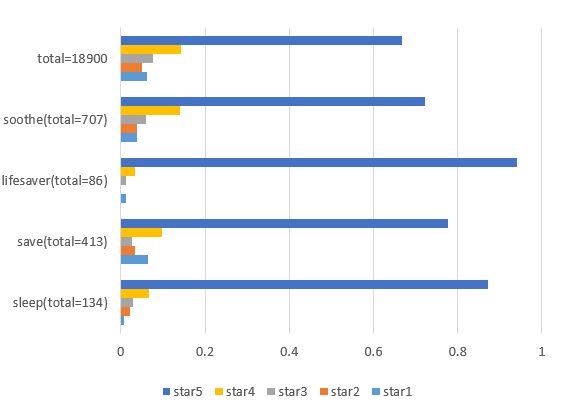
\includegraphics[width=5cm,height=5cm]{figures/pos-p.png}
	}
	\subfigure[Negative words]{
		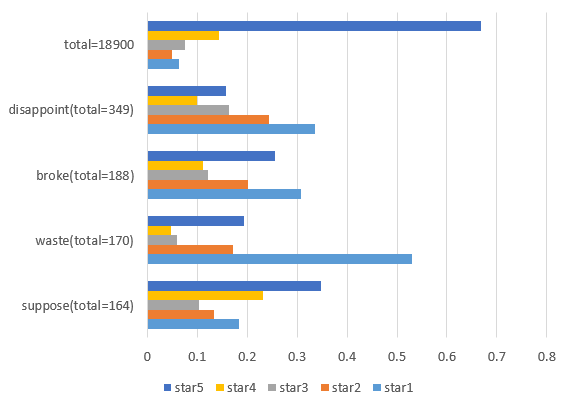
\includegraphics[width=5cm,height=5cm]{figures/neg-p.png}
	}
	\caption{Pacifier}
\end{figure}

\newpage
As it can be seen from the chart that although some reviews contained positive words are associate with lower star rating because of sentence like this"This product is not that prefect", on the whole, whether it is a hair\_dryer, microwave oven or pacifier, reviews that contain positive words are generally correspond to higher star ratings(the total number of four-star reviews and five-star reviews are over 75\%). Also, comments that contain negative words are generally associated with lower star ratings(the total number of one-star reviews and two-star reviews are also over 75\%). In summary, those specific quality descriptors of text\-based reviews are strongly associated with rating levels.



\newpage
\section{Letter for the Director}
\noindent Date: March 9, 2020

\noindent To: Sunshine Company Marketing Director

\noindent From: MCM Team \#2011260

\noindent Subject: Amazon Review Analysis

\noindent \hrulefill

\noindent Dear Marketing Director:

It is our pleasure to use our knowledge to help your company. We have performed a series of analysis and processing using the data provided by your company and obtained some meaningful results. We sincerely hope that our work can help your company. The datils of our work are as follows:

First of all, we identified some useful information from the data set. The first information is that we find that this three types of goods will have higher sales in January, February, July, August, and December, also lower sales in May, June, September, and October. The second information shows that people are more willing to decide whether to buy this product based on the content of one-star and five-star reviews. The content of reviews did not influence people's buying decisions that much.

Secondly, we combined the two product measurement standards of consumer reviews and star ratings in the data provided by your company, and obtained a comprehensive evaluation standard. This evaluation standard is more easy to understand than consumer reviews and more comprehensive than star ratings. We use natural language processing technology to quantify consumer reviews and multiply them with star ratings, then divide by the sum of all consumer reviews after quantification to reduce errors. We believe that using such data measure method will give your company the most detailed product review information.

After that, we use the data measure method obtained previously to calculate the changes of the reputation of product in the online marketplace over time. We found that the trend of the change of product reputation has the same thing in common, that is, it first increases, then decreases, and eventually stabilizes. At the same time, we combine the changes of the reputation of the product and the measures we have established before to identify those reviews that can best predict the success of the product. We found that when the quality of the review reaches a certain level, a higher star rating indicates the future success of the product, and a lower star rating indicates the future failure of the product. If the written review does not reach that level, then this review cannot be used to predict the success of the product.

Finally, we analyzed the relationship between specific quality descriptors and rating levels in text-based reviews. Our analysis found that these specific quality descriptors are closely related to rating levels. In most case, those descriptors that are positive like "smooth" for hair\_dryer, "fit" for microwave oven, "sleep" and "lifesaver" for pacifier, are associated with higher rating levels. In contrast, those descriptors that are negative are associated with lower rating levels.

Of all our work, we are most confident on the task of predicting the success of a product, because in this work we considered all the information about the consumer's evaluation of a product, and design accurate review screening standard. Through our work, your company can accurately locate the most valuable evaluations from thousands of evaluations, and accurately predict the success of the product.

Finally, thank you again for this opportunity. We sincerely hope that our work can help your company.

Best,

MCM Team \#2011260

\newpage
\begin{thebibliography}{99}
\bibitem{1}Ramos, Juan. "Using tf-idf to determine word relevance in document queries." Proceedings of the first instructional conference on machine learning. Vol. 242. 2003.
\bibitem{2}Saldaña, Zoë Wilkinson. "Sentiment Analysis for Exploratory Data Analysis." Programming Historian (2018).  
\bibitem{3}Fenech, Jean-Pierre, Ying Kai Yap, and Salwa Shafik. "Brief Technical Note: A Markov Chain Approach to Measure Investment Rating Migrations." Australasian Accounting, Business and Finance Journal 7.3 (2013): 145-154.  
\bibitem{4}Dave K, Lawrence S, Pennock D M. Mining the peanut gallery: Opinion extraction and semantic classification of product reviews[C]//Proceedings of the 12th international conference on World Wide Web. ACM, 2003: 519-528. 
\bibitem{5}Dellarocas, Chrysanthos. "The digitization of word of mouth: Promise and challenges of online feedback mechanisms." Management science 49.10 (2003): 1407-1424. 
\bibitem{6}Liu, Jingjing, et al. "Low-quality product review detection in opinion summarization." Proceedings of the 2007 Joint Conference on Empirical Methods in Natural Language Processing and Computational Natural Language Learning (EMNLP-CoNLL). 2007. 
\bibitem{7}Weimer M, Gurevych I. User Automatically Assessing The Post Quality In Online Discussions on Software[C]. Proceedings of The 45th Annual Meeting of the ACL on Interactive,2007:125-128.
\bibitem{8}Dellarocas C, Zhang X Q, Awad N F. Exploring The Value of Online Product Reviews in Forecasting Sales: The Case of Motion Pictures [J].Journal of 
Interactive Marketing ,2007,21(4):23-45.
\bibitem{9} Cal Q, Duan W, Gan Q. Exploring Determinants of Voting For The “Helpfulness” of Online User Reviews: A Text Mining Pproach[J].Dicision Support Systems,2011,50(2):511-521. 
\end{thebibliography}



%\begin{appendices}
%
%\section{First appendix}
%
%In addition, your report must include a letter to the Chief Financial Officer (CFO) of the Goodgrant Foundation, Mr. Alpha Chiang, that describes the optimal investment strategy, your modeling approach and major results, and a brief discussion of your proposed concept of a return-on-investment (ROI). This letter should be no more than two pages in length.
%
%\begin{letter}{Dear, Mr. Alpha Chiang}
%
%\lipsum[1-2]
%
%\vspace{\parskip}
%
%Sincerely yours,
%
%Your friends
%
%\end{letter}
%Here are simulation programmes we used in our model as follow.\\
%
%\textbf{\textcolor[rgb]{0.98,0.00,0.00}{Input matlab source:}}
%\lstinputlisting[language=Matlab]{./code/mcmthesis-matlab1.m}
%
%\section{Second appendix}
%
%some more text \textcolor[rgb]{0.98,0.00,0.00}{\textbf{Input C++ source:}}
%\lstinputlisting[language=C++]{./code/mcmthesis-sudoku.cpp}
%
%\end{appendices}
\end{document}
%%
%% This work consists of these files mcmthesis.dtx,
%%                                   figures/ and
%%                                   code/,
%% and the derived files             mcmthesis.cls,
%%                                   mcmthesis-demo.tex,
%%                                   README,
%%                                   LICENSE,
%%                                   mcmthesis.pdf and
%%                                   mcmthesis-demo.pdf.
%%
%% End of file `mcmthesis-demo.tex'.
